\chapter{Двигатель постоянного тока 2.0}
\label{ch:chap2}

Уравнения двигателя постоянного тока независимого возбуждения, но покруче:
$$
  J\dot{\omega} = M, \tab M=k_mI, \tab I = \frac{U + \epsilon}{R}, 
$$
$$
\tab \epsilon = \epsilon_i + \epsilon_s, \tab \epsilon_i = -k_e\omega ,\tab \epsilon_s = - L\dot{I}
$$

В случае моего второго варианта константы:
$$
  k_m = 0.3239, \tab k_e = 0.3239, \tab J =0.0018, \tab R =4.6916, \tab L =1.1682, 
$$

В нашем случае мы считаем напряжение $U(t)$ - входом объекта, а на выходе $\omega(t)$ - угловая скорость.

\section{Передаточная функция}
Из-за появления индуктивности дифференциальное уравнение немного усложнится:
$$
\ddot{\omega} + \frac{R}{L}\dot{\omega} + \frac{k_m k_\epsilon}{LJ}\omega = \frac{k_m}{LJ}U
$$
Из него мы получаем следующее:
$$
\omega = \frac{k_m}{JL}\frac{1}{s^2 + \frac{R}{L}s + \frac{k_m k_\epsilon}{LJ}}[U]
$$
Немного причешем уравнение, получаем передаточную функцию:
$$
\omega = \frac{k_m}{JLs^2 + JRs + k_m k_\epsilon}[U]
$$
Полученное можно привести к общему виду - колебательного звена:
$$
W(s) = \frac{K}{T^2 s^2 + 2\xi Ts + 1}
$$
Тогда константы $K, T, \xi$ в нашем случае будут равны:
$$
 K= \frac{1}{k_e} \approx 3.08, \tab T = \sqrt{\frac{LJ}{k_m k_\epsilon}}\approx 0.14, \tab \xi = \frac{R}{2}\sqrt{\frac{J}{L k_m k_\epsilon}} \approx 0.28
$$
Также $\xi$ называют коэффициентом демпфирования $\in (0; 1)$ для колебательного звена.

\section{Временные  характеристики}

$$
y_{i.r.}(t) = \mathcal{L}^{-1}\{W(s)\}
$$
$$
y_{s.r.}(t) = \mathcal{L}^{-1}\{W(s)\cdot \frac{1}{s}\}
$$

Начнём с весовой функции, для неё обернём константы в новые переменные, а после аккуратно выделим полный квадрат, чтобы получить табличную формулу обратного преобразования Лапласа:
$$
  W(s) = \frac{K}{T^2(s^2 + 2\frac{\xi}{T}s + \frac{1}{T^2})} = \frac{K}{T^2}\frac{1}{(s + \frac{\xi}{T})^2 + \frac{1-\xi^2}{T^2}} = \frac{K}{T^2}\frac{\sqrt{\frac{1-\xi^2}{T^2}}}{((s + \frac{\xi}{T})^2 + \frac{1-\xi^2}{T^2})\sqrt{\frac{1-\xi^2}{T^2}}}
$$
$$
  y_{i.r.} = \mathcal{L}^{-1}\{W(s)\} = \frac{K}{T^2} \mathcal{L}^{-1}\bigg\{\frac{\sqrt{\frac{1-\xi^2}{T^2}}}{((s + \frac{\xi}{T})^2 + \frac{1-\xi^2}{T^2})\sqrt{\frac{1-\xi^2}{T^2}}}\bigg\} = \frac{K}{T^2} \frac{e^{-\frac{\xi}{T}t}sin(\sqrt{\frac{1-\xi^2}{T^2}}t)}{\sqrt{\frac{1-\xi^2}{T^2}}}
$$

Для переходной функции немного сложнее, придётся немного больше поиграться с формулами:
$$
  \begin{aligned}
    W(s) = \frac{K}{sT^2(s^2 + 2\frac{\xi}{T}s + \frac{1}{T^2})} = K\bigg(\frac{1}{s} - \frac{T^2s+2\xi T}{T^2s^2 +2\xi Ts + 1}\bigg)  \\
    = K\bigg(\frac{1}{s} - \frac{s+2\frac{\xi}{T}}{s^2 +2\frac{\xi}{T}s + \frac{1}{T^2}}\bigg) = K\bigg(\frac{1}{s} - \frac{s+2\frac{\xi}{T}}{(s + \frac{\xi}{T})^2 + \frac{1-\xi^2}{T^2}}\bigg) = \\
    K\bigg(\frac{1}{s} - \frac{s+\frac{\xi}{T}}{(s + \frac{\xi}{T})^2 + \frac{1-\xi^2}{T^2}} - \frac{\frac{\xi}{T}}{(s + \frac{\xi}{T})^2 + \frac{1-\xi^2}{T^2}}\bigg) = 
  \end{aligned}
$$
$$
  \begin{aligned}
    y_{s.r.} = \mathcal{L}^{-1}\{W(s)\cdot\frac{1}{s}\} = \\
    K \bigg(\mathcal{L}^{-1}\{\frac{1}{s}\} - \mathcal{L}^{-1}\{  \frac{s+\frac{\xi}{T}}{(s + \frac{\xi}{T})^2 + \frac{1-\xi^2}{T^2}} \} - \mathcal{L}^{-1}\{  \frac{\frac{\xi}{T}}{(s + \frac{\xi}{T})^2 + \frac{1-\xi^2}{T^2}} \} \bigg) = 
    \\K - Ke^{-\frac{\xi}{T}t}cos(\sqrt{\frac{1-\xi^2}{T^2}})- \frac{Ke^{-\frac{\xi}{T}t}sin(\sqrt{\frac{1-\xi^2}{T^2}})\frac{\xi}{T}}{\sqrt{\frac{1-\xi^2}{T^2}}} 
  \end{aligned}
$$

\newpage
\begin{figure}[ht]
  \centering
  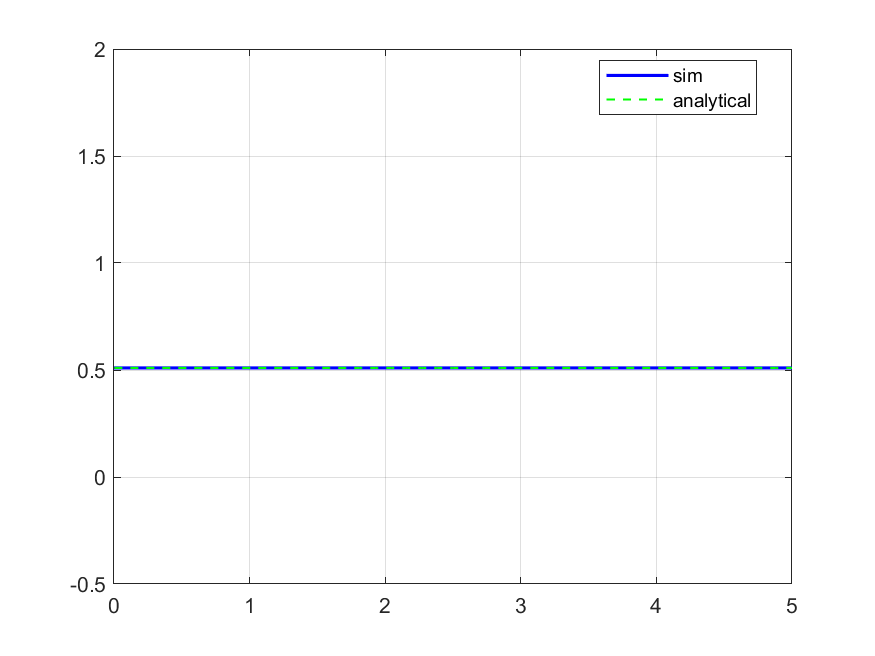
\includegraphics[width=0.8\textwidth]{impulse_responce5.png}
  \caption{Воздействие - \textrm{impulse responce}}
\end{figure}

\begin{figure}[ht]
    \centering
    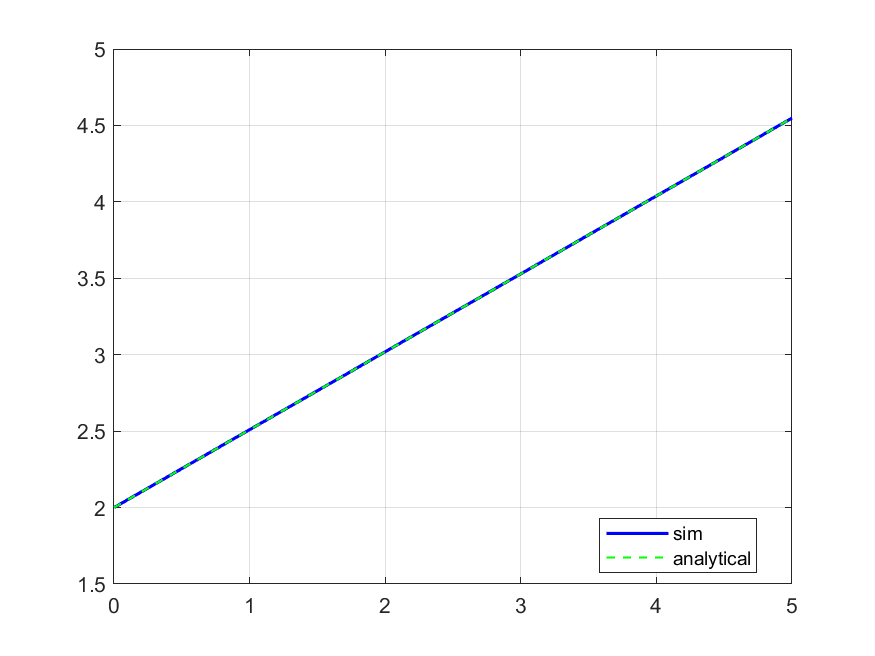
\includegraphics[width=0.8\textwidth]{step_responce5.png}
    \caption{Воздействие - \textrm{step responce}}
  \end{figure}
\newpage

\section{Частотные характеристики}

$$
W(j\omega) =  \frac{K}{T^2(j\omega)^2 + 2\xi T(j\omega) + 1} = \frac{K}{\bigg(1 - T^2\omega^2\bigg) + \bigg(2\xi Tj\omega\bigg)} = 
$$

$$
  K\frac{ 1 - T^2\omega^2 -  j2\xi T\omega}{ (1 - T^2\omega^2)^2 + (2\xi T\omega)^2 } =  
$$

$$
K\bigg(\frac{ 1 - T^2\omega^2 }{ (1 - T^2\omega^2)^2 + (2\xi T\omega)^2 } - j\frac{2\xi T\omega}{ (1 - T^2\omega^2)^2 + (2\xi T\omega)^2 }\bigg)
$$
Амплитудно-частотная характеристика:
$$
A(\omega) = \sqrt{P^2 + Q^2} = \sqrt{ \frac{ K((1 - T^2\omega^2)^2 + (2\xi T\omega)^2) }{ \bigg((1 - T^2\omega^2)^2 + (2\xi T\omega)^2\bigg)^2 }  }
$$
$$
A(\omega) = \frac{ K }{ \sqrt{ \bigg((1 - T^2\omega^2)^2 + (2\xi T\omega)^2\bigg) }  }
$$

Логарифмическая-Амплитудно-частотная характеристика:
$$
L(\omega) = 20lg(A) = 20lg(K) - 10lg( (1 - T^2\omega^2)^2 + (2\xi T\omega)^2 ) 
$$
Фазовая-частотная характеристика:
$$
\phi(\omega) = atan2(Q,P) = -atan2( 2\xi T\omega , 1 - T^2\omega^2)
$$
\newpage
\begin{figure}[ht]
  \centering
  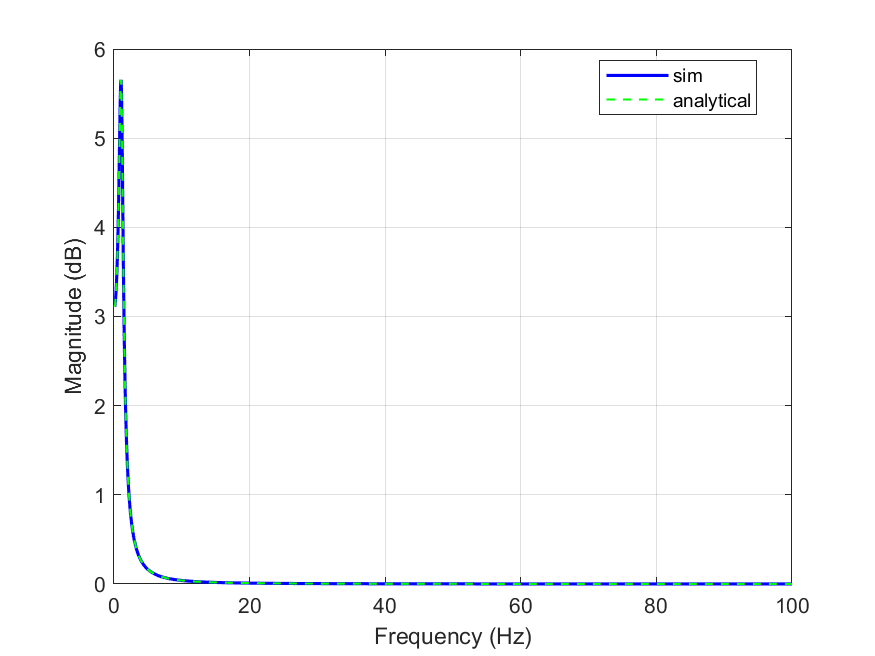
\includegraphics[width=0.8\textwidth]{freq_ampl2.png}
\caption{Сравнение - АЧХ}
\end{figure}

\begin{figure}[ht]
    \centering
    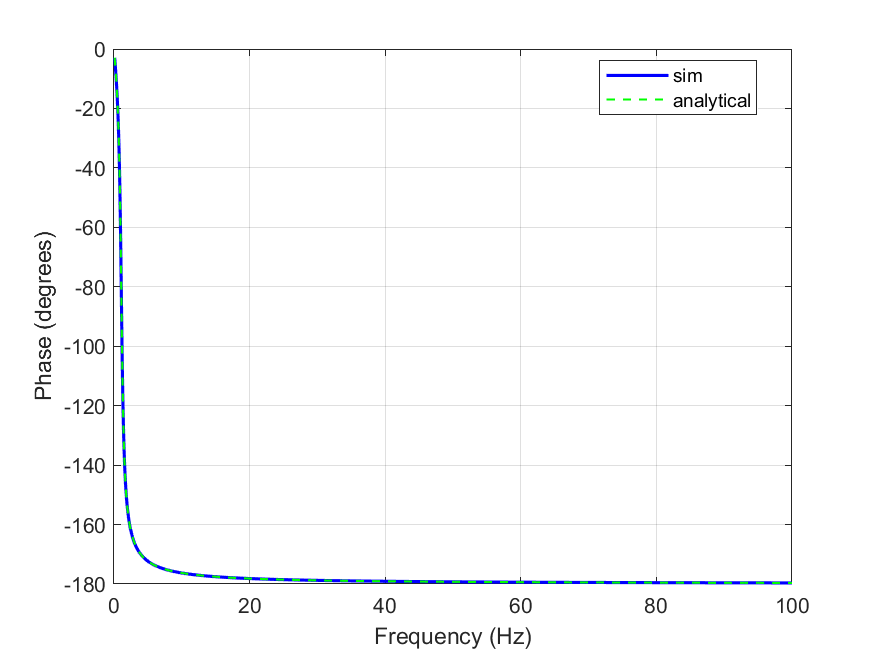
\includegraphics[width=0.8\textwidth]{freq_phase2.png}
  \caption{Сравнение - ФЧХ}
  \end{figure}
\newpage
\begin{figure}[ht]
    \centering
    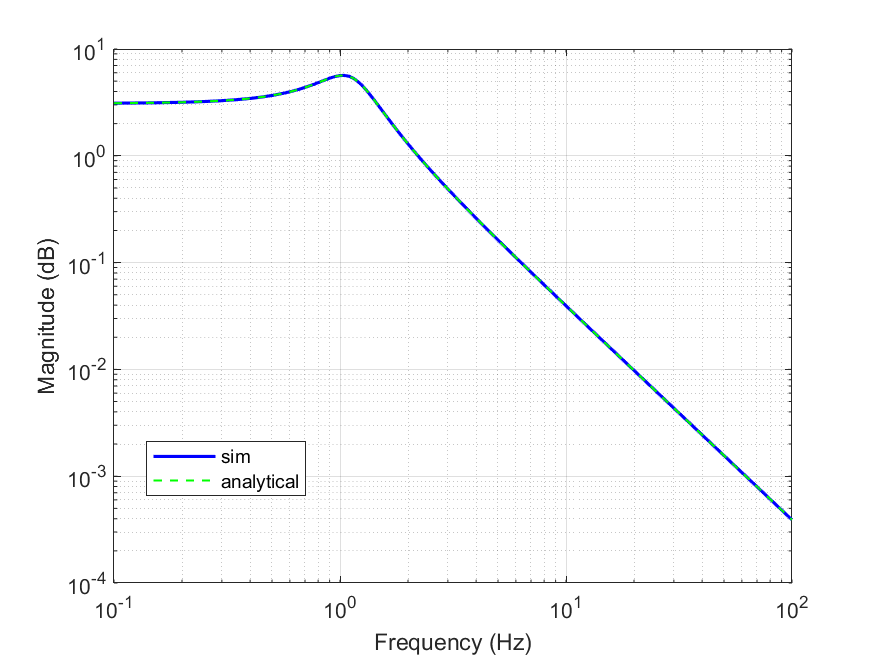
\includegraphics[width=0.8\textwidth]{lfreq_ampl2.png}
  \caption{Сравнение - ЛАЧХ}
  \end{figure}
  
  \begin{figure}[ht]
      \centering
      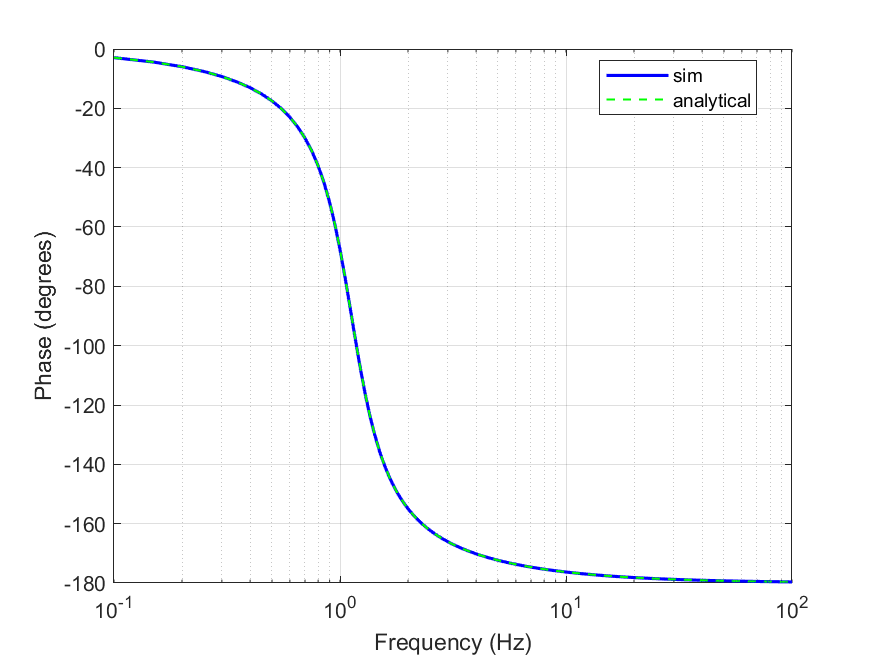
\includegraphics[width=0.8\textwidth]{lfreq_phase2.png}
    \caption{Сравнение - ЛФЧХ}
    \end{figure}

    % \begin{figure}[ht]
    %   \centering
    %   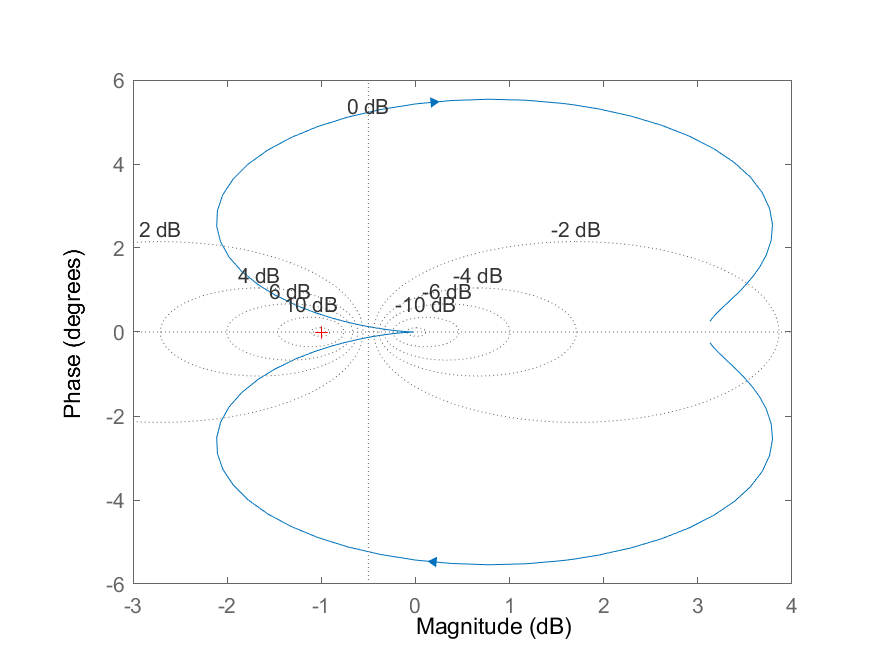
\includegraphics[width=0.8\textwidth]{nyquist2.png}
    % \caption{АФЧХ}
    % \end{figure}
\newpage


\endinput